% Intended LaTeX compiler: xelatex
\documentclass[10pt,a4paper]{article}
\usepackage{graphicx}
\usepackage{longtable}
\usepackage{wrapfig}
\usepackage{rotating}
\usepackage[normalem]{ulem}
\usepackage{capt-of}
\usepackage{hyperref}
\usepackage[a4paper,margin=1.25cm]{geometry}
\usepackage{xcolor}
\usepackage{fontspec}
\usepackage{graphicx}
\usepackage{enumitem}
\usepackage{tabularx}
\usepackage{titlesec}
\usepackage{microtype}
\usepackage[british,UKenglish,USenglish,american]{babel}
\usepackage[autostyle=true]{csquotes}

\definecolor{cvaccent}{RGB}{100, 14, 39}
\definecolor{cvtext}{RGB}{35, 35, 35}
\definecolor{cvmuted}{RGB}{82, 82, 82}

\setmainfont[
Path = ../curriculum-vitae/Fonts/MinionPro/,
Extension = .otf,
UprightFont = *_Regular,
ItalicFont = *_It,
BoldFont = *_Bold,
BoldItalicFont = *_BoldIt,
Ligatures=TeX]{MinionPro}

\setsansfont[
Path = ../curriculum-vitae/Fonts/MyriadPro/,
Extension = .otf,
UprightFont = *_Regular,
ItalicFont = *_It,
BoldFont = *_Bold,
BoldItalicFont = *_BoldIt,
Ligatures=TeX]{MyriadPro}

\hypersetup{
  pdfcreator={XeLaTeX},
  pdftitle={Ruhila Goswami Two-Page CV},
  colorlinks=true,
  urlcolor=cvaccent,
  linkcolor=cvaccent,
  citecolor=cvaccent
}

\pagestyle{empty}
\setlength{\parindent}{0pt}
\setlength{\parskip}{0.12em}
\setlist[itemize]{nosep,leftmargin=1.2em}
\titleformat{\section}{\large\sffamily\bfseries\color{cvaccent}}{}{0pt}{}[\vspace{-0.35em}\titlerule]
\titlespacing*{\section}{0pt}{0.65em}{0.35em}

\newcommand{\sectionspace}{\vspace{0.25em}}
\newcommand{\entry}[4]{%
  \textbf{#1}\hfill{\small\color{cvmuted}#2}\\%
  {\small\color{cvmuted}#3}\\[-0.15em]%
  #4\par\sectionspace}
\newcommand{\shortentry}[3]{%
  \textbf{#1}\hfill{\small\color{cvmuted}#2}\\[-0.1em]%
  #3\par\sectionspace}
\newcommand{\skillline}[2]{\textbf{#1:} #2\par}

\date{}
\title{}
\begin{document}

\begin{minipage}[t]{0.76\textwidth}
{\Huge\sffamily\bfseries Ruhila Goswami}\\[-0.15em]
{\color{cvmuted}Previous name: Ruhila S. \textbullet{} Date of Birth: 20.09.2001}\\
\href{mailto:ruhila@ieee.org}{ruhila@ieee.org} \textbullet{} \href{https://github.com/RuhiRG}{github.com/RuhiRG}\\[-0.1em]
{\itshape ``Nothing exists for itself alone, but only in relation to other forms of life.'' -- Charles Darwin}
\end{minipage}
\hfill
\begin{minipage}[t]{0.18\textwidth}
\raggedleft
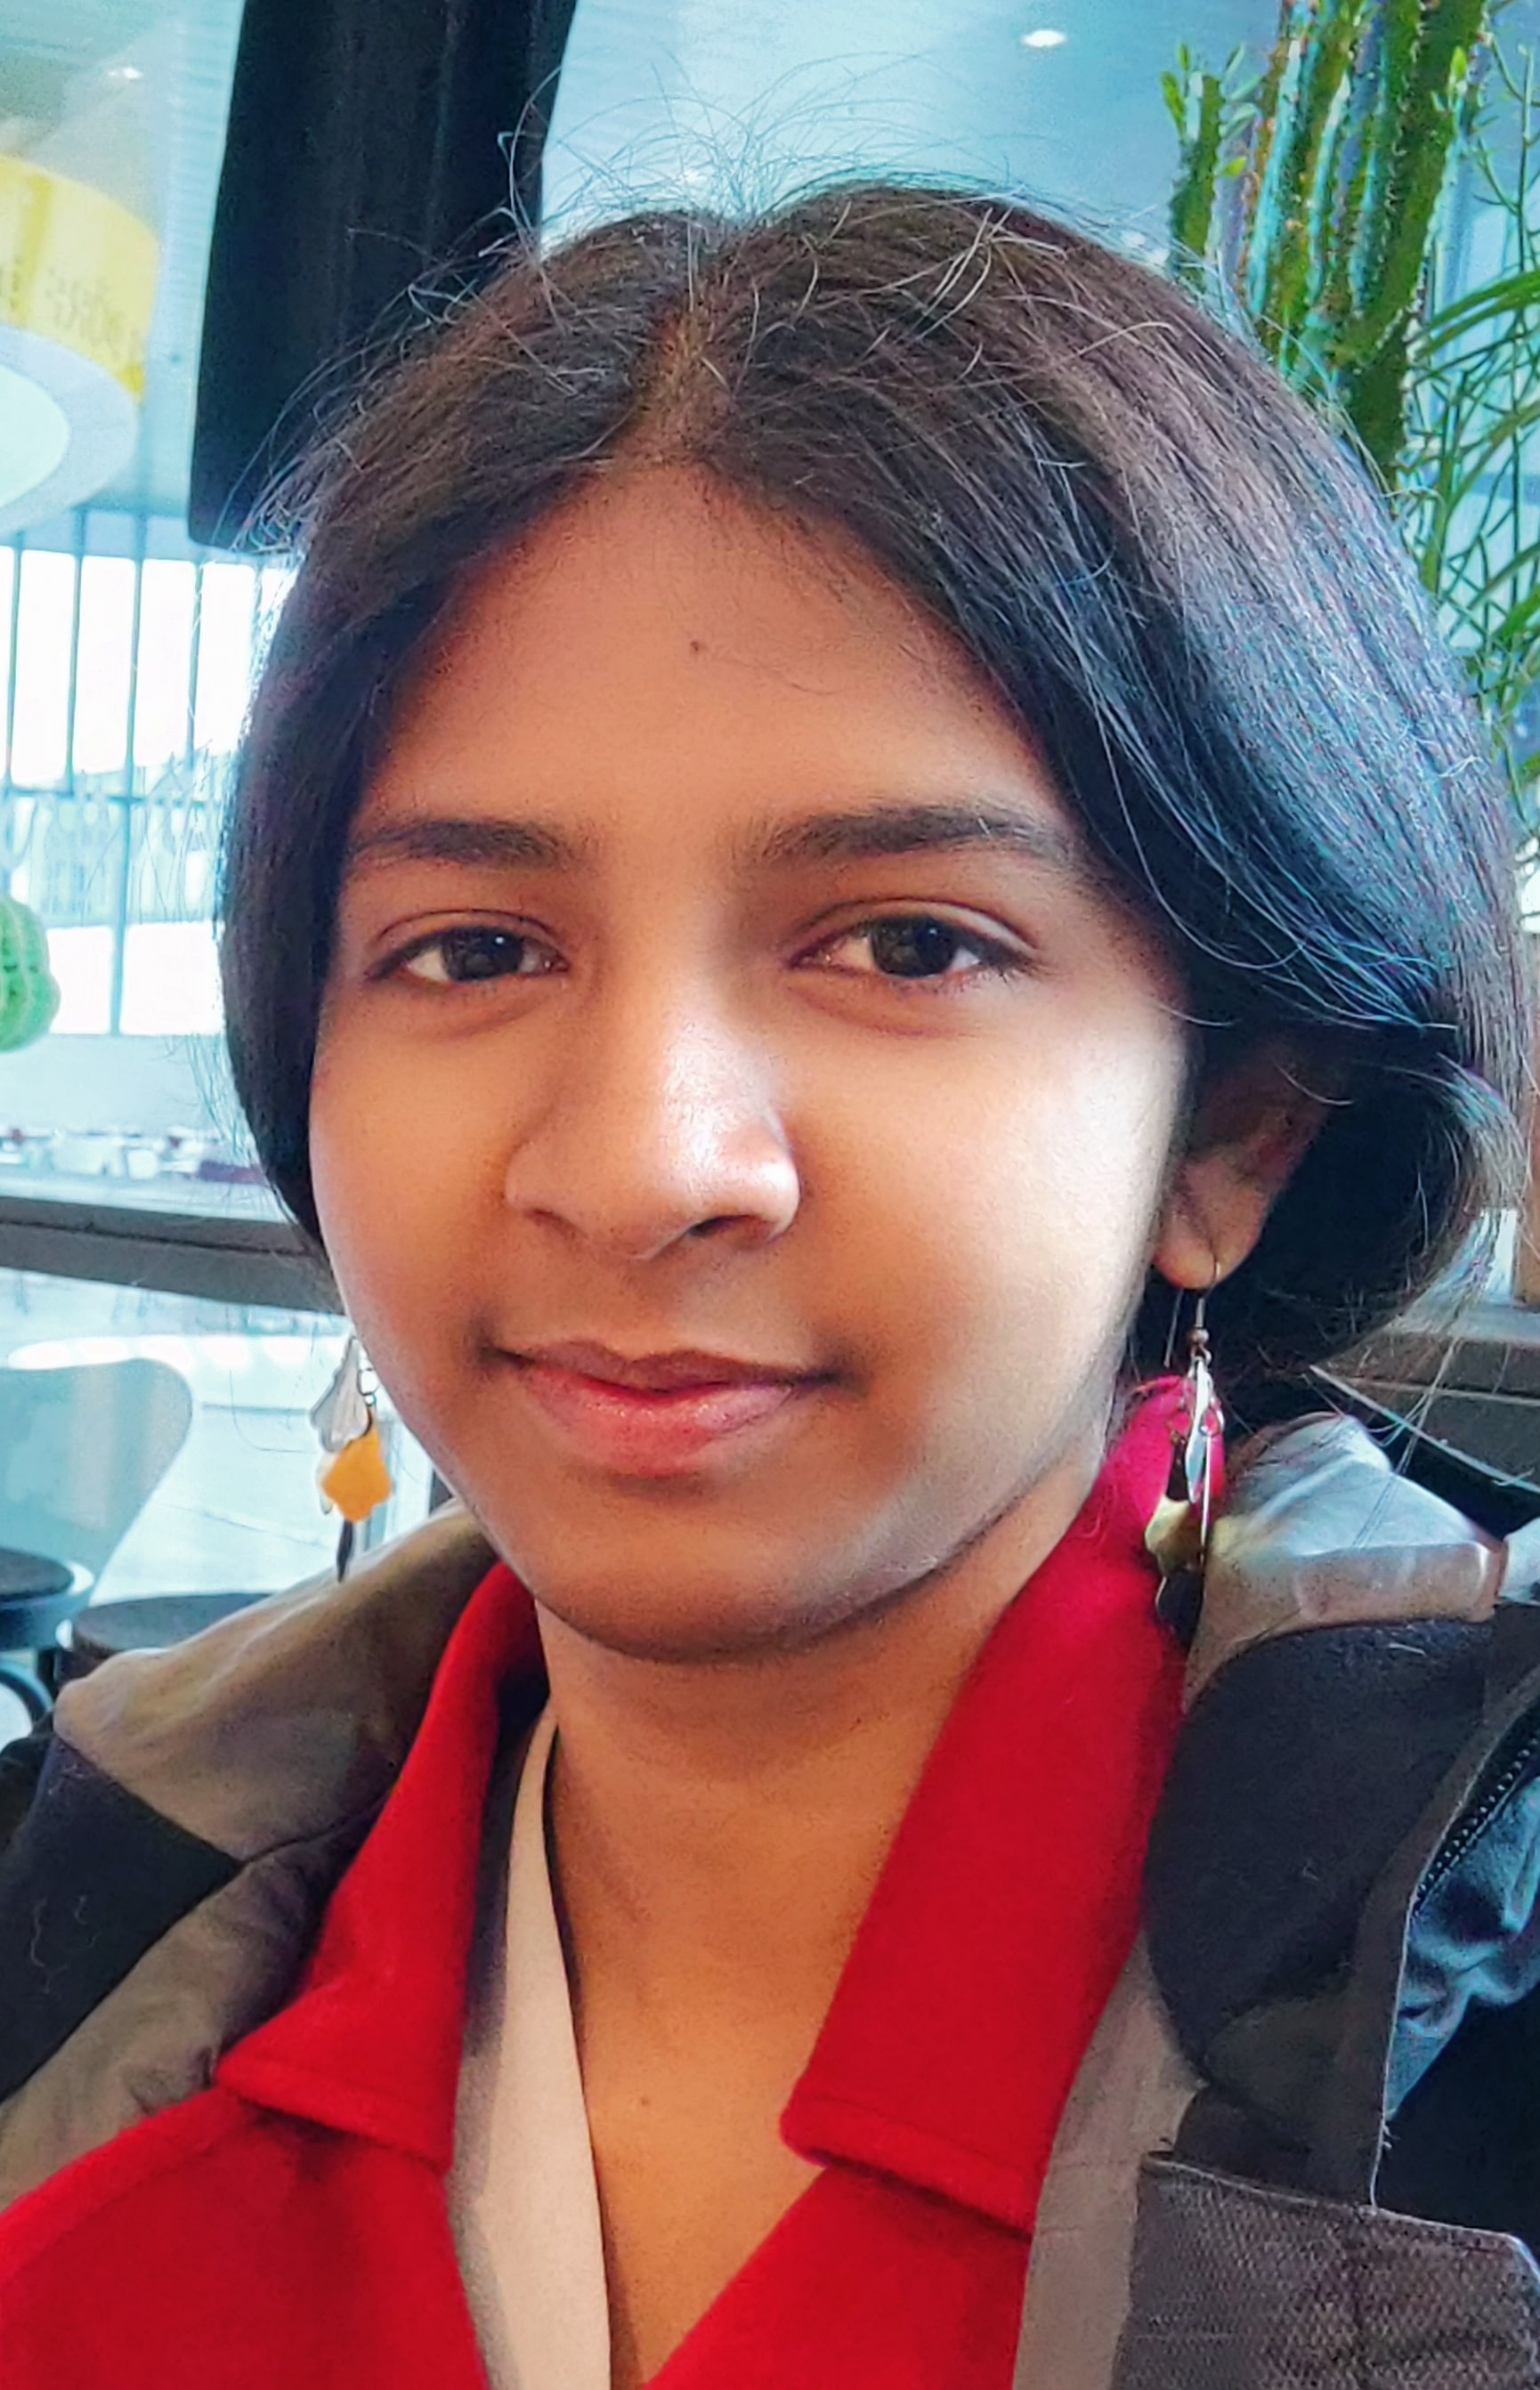
\includegraphics[width=2.35cm,height=2.35cm,keepaspectratio]{../curriculum-vitae/Picture/ruhi.jpeg}
\end{minipage}

\section{Research Profile}
\skillline{Focus}{Evolutionary divergence and dental variation in salmonids.}
\skillline{Interests}{Population genetics; phenotypic-genotypic mapping; structural variation in genomes and selection; salmonid evolution; non-invasive methods.}
\skillline{Methods}{Phylogenetic inference, genomic synteny, PCR-based sex determination, skeletal phenotyping, field sampling, and reproducible analysis in R and Python.}

\section{Education}
\entry{University of Iceland}{2024--2026}{M.S. Biological Science, Reykjavík, Iceland}{Advisor: Prof. Arnar Pálsson. \textsc{Thesis:} Evolutionary Divergence in Dental Variation and Sex Chromosome Architecture in Icelandic Brown Trout and Arctic Charr.}
\entry{IISER Mohali}{2021--2024}{B.S. Biology (Major), India}{First Division with Honors.}

\section{Research Experience}
\entry{University of Iceland}{Summer 2023}{Research Staff with Prof. Arnar Pálsson}{Studied synteny of histone genes in salmonids, focusing on gene arrangement and neighboring genomic regions.}
\entry{University of Iceland}{Summer 2022}{Research Staff with Prof. Arnar Pálsson}{Reproducible phylogenetic workflow for possible molecular evolutionary pathways in salmonids: NCBI data curation, BLAST homology inference, MUSCLE5 alignments, Gblocks trimming, and BIONJ/RAxML-NG tree simulation. \textsc{Project Report:} Computational Primitives for Evolutionary Paths ($\approx 147$ pages).}
\entry{IIT Kanpur}{Winter 2022}{Research Interns with Prof. Debabrata Goswami and Dr. Nagma Parveen}{Studied non-linear optics, optical tweezers, viral wet-lab methods, and a SARS-CoV-2 pseudovirus protocol using an HIV-1 lentiviral packaging system.}
\entry{IISER Mohali}{Summer 2021}{Research Intern with Dr. Lolitika Mandal}{Explored genetic tools for \textit{Drosophila} from a wet-lab perspective of data collection and analysis.}

\section{Publications, Posters, and Awards}
\shortentry{Manuscript in preparation}{2026}{Evolutionary divergence in tooth numbers and bone shape by populations and species in Icelandic salmonids.}
\shortentry{Posters}{2025--2026}{Icelandic Ecological Society (Vistís), NOWPAS, and IceBio posters on tooth numbers and bone shape in Icelandic salmonids; Best Poster Award at Vistís 2025.}
\shortentry{Selected proceedings and presentations}{2022}{IEEE PDGC proceedings on reproducible literate phylogenetic analysis and high-performance computing workflows; BES poster on \textit{Salmo salar} histone sequence data.}

\section{Teaching}
\shortentry{LÍF401G Developmental Biology}{Spring 2026}{Teaching Assistant, University of Iceland. Course led by Prof. Adam Ray Smith; assisted with embryo analysis.}
\shortentry{LÍF541G Plant Physiology}{Fall 2025}{Teaching Assistant, University of Iceland. Course led by Prof. Victor Anthony Albert; led student discussions in a course focused primarily on plant genetics.}
\shortentry{LÍF403G Evolutionary Biology}{Spring 2025}{Teaching Assistant, University of Iceland; undergraduate course on evolutionary theory, natural selection, adaptation, and the history of life.}

\section{Research Skills}
\skillline{Genomics}{Population genetics, genomic synteny, structural variation, PCR-based sex determination, non-invasive sampling.}
\skillline{Phenotypes and fieldwork}{Dental and craniofacial variation, bone extraction, otolith extraction, fish dissection, electrofishing, salmonid sampling and preservation.}
\skillline{Evolutionary methods}{Phylogenetic tree construction (distance, maximum likelihood, Bayesian), BLAST, MUSCLE5, Gblocks, RAxML-NG, BEAST2.}
\skillline{Computing and lab}{R, Python, shell, Git, Snakemake, reproducible literate programming, DNA extraction and preservation, PCR, microscopy, \textit{Drosophila} tissue dissection, cell culture.}

\section{Service, Open Source, and Affiliations}
\shortentry{Google Summer of Code}{2023--2024}{Student Developer on Python bindings and documentation for d-SEAMS/pySEAMS, including installation refinements, usability improvements, and repository maintenance.}
\shortentry{IEEE P3173}{2022--present}{Secretary, IEEE Standards Committee for Endocrine Disrupting Chemical Hazard Labeling.}
\skillline{Memberships}{Nordic Society Oikos; Icelandic Ecological Society (Vistís); Icelandic Biological Society (Líffræðigáttin); British Ecological Society; Genetics Society, UK; Genetics Society of America.}
\end{document}
